\documentclass{beamer}
\renewcommand\thesection{\arabic{section}}
\newcommand{\myfont}{\rmfamily\normalsize\upshape\mdseries}
\newcommand{\degree}{^\circ}
\title{\sffamily Review IV(Slides 170 - 250)}
\subtitle{\textbf{Real Functions}\\ }
\institute[UM-SJTU JI]{University of Michigan-Shanghai Jiao Tong University Joint Institute}
\author{HamHam}
\usepackage{graphicx}
\usepackage{picinpar}
\usepackage{indentfirst}
\usepackage{chemformula}
\usepackage{geometry}
\usepackage{subfigure}
\usepackage{appendix}
\usepackage{amsfonts,amsmath,amssymb}
\usepackage{enumerate}
\usepackage{float}
\usepackage{geometry}
\usepackage{latexsym}
\usepackage{listings}
\usepackage{multicol,multirow,multido}
\usepackage{tabularx}
\usepackage{ulem}
\usepackage{tikz}
\usepackage{xcolor}
\usepackage{cite}
\usepackage{setspace}
\usepackage{hyperref}
\usepackage{textpos}
\usepackage{booktabs}

\usetheme[dove]{Boadilla}
\usecolortheme{dolphin}
\useoutertheme{miniframes}
\begin{document}
    \usebackgroundtemplate{\tikz\node[opacity=0.3]{
    
\includegraphics[width=\paperwidth,
    height=\paperheight]{hamster.jpg}
    };}
\begin{titlepage}
    \begin{center}
        VV186 - Honors Mathmatics II
    \end{center}
\end{titlepage}
\myfont
\section{Real Func.}
\begin{frame}
    \frametitle{Common Types \& Manipulating Functions}
    Common function types (these should be familiar from high school):
    \begin{itemize}
        \item Power functions: $x^n$
        \item Polynomials: Combinations of power functions
        \item Rational functions: Quotient of polynomials
        \item Piecewise functions: ”sticking” functions together 
        \item Periodic functions: $f(x + T) = f(x)$
    \end{itemize}
    Manipulating functions (also familiar from high school):
    \begin{itemize}
        \item  $f(k \cdot x)$
        \item $k \cdot f(x)$
        \item  $f(x + t)$
        \item $f(x) + t$
    \end{itemize}
\end{frame}
\begin{frame}
    \frametitle{Addition, Multiplication and Composition}
    Let $f:X_1 \to Y_1, g:X_2 \to Y_2 ,$ and let $E=X_1 \bigcap X_2$, then
    $$f+g:=f(x)+g(x),x \in E$$
    $$f \cdot g :=f(x) \cdot g(x), x \in E$$
    \begin{center}
    $f \circ g : X_2 \to Y_1, x \mapsto f(g(x)),$ \textcolor{red}{if $g(x)\in Y_2 \cap X_1 \neq \emptyset$}
    \end{center}
\end{frame}
\begin{frame}
    \frametitle{Some terms..}
    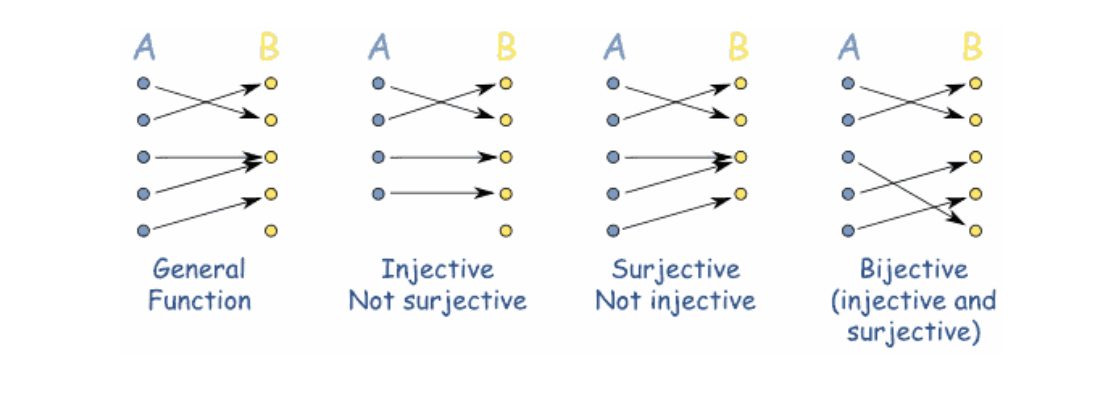
\includegraphics[width=1\textwidth]{sur.png} 
    Try to remember it...perhaps?   
\end{frame}
\section{Limit}
\begin{frame}
    \frametitle{Limit}
    Two Definitions:
    \begin{itemize}
        \item[(1)] (Common) Let $f$ be a real- or complex-valued function defined on a subset $\Omega\subset \mathbb{R}$ 
        and let $x_0$ be an accumulation point of $f$. Then the limit of $f$ as $x\to x_0$ is equal to $L \in \mathbb{C}$, written 
        $$\underset{x\to x_0}{\lim} ⁡f(x) = L :\Leftrightarrow\underset{\delta>0}{\exists}~\underset{x\in \Omega\backslash\{x_0\}}{\forall} |x-x_0|<\delta\Rightarrow|f(x)-L|<\varepsilon$$
        \item[(2)] (Sequential) Let $f$ be a real- or complex-valued function defined on a subset $\Omega\subset \mathbb{R}$ 
        and let $x_0$ be an accumulation point of $f$. Then the limit of $f$ as $x\to x_0$ is equal to $𝐿 \varepsilon \mathbb{C}$, written 
        $$\underset{x\to x_0}{\lim} ⁡f(x) = L :\Leftrightarrow\underset{a_n\subset \Omega}{\forall}~a_n\to x_0 \Rightarrow f(a_n)\to L$$
    \end{itemize} 
\end{frame}

\begin{frame}
    \frametitle{Common Results}

    Let $f, g$ be two real functions with the same domain $\Omega\subset\mathbb{R}$. 
    Furthermore, suppose $\underset{x\to x_0}{\lim} ⁡f(x)$ and $\underset{x\to x_0}{\lim}⁡g(x)$ 
    exists at some point $x_0\in \Omega$. Then:
    \begin{itemize}
        \item $\underset{x\to x_0}{\lim} [⁡f(x)+g(x)]= \underset{x\to x_0}{\lim} ⁡f(x)+ \underset{x\to x_0}{\lim}⁡g(x)$
        \item $\underset{x\to x_0}{\lim} [⁡f(x)\cdot g(x)]= \underset{x\to x_0}{\lim} ⁡f(x)\cdot \underset{x\to x_0}{\lim}⁡g(x)$
        \item $\underset{x\to x_0}{\lim} [⁡f(x)/ g(x)]= \underset{x\to x_0}{\lim} ⁡f(x)/ \underset{x\to x_0}{\lim}⁡g(x)$, if $\underset{x\to x_0}{\lim}⁡g(x)\neq 0$
    \end{itemize} 
    \vspace{2em}
    (You are encouraged to prove these results, the proof is similar for that of sequence)
\end{frame}
\begin{frame}
    \frametitle{Landau Symbols}
    My interpretation:
    \begin{itemize}
        \item Big-O : \textcolor{red}{As Large As...}
        $$f(x)=O(\phi(x)),x\to \infty: \underset{C>0}{\exists}~\underset{M>L}{\exists}~x>M~\Rightarrow |f(x)|\leq C|\phi(x)|$$
        \item Small-o : \textcolor{blue}{To Small so I don't care at all}
        $$f(x)=o(\phi(x)),x\to x_0: \underset{C>0}{\forall}~\underset{\varepsilon>0}{\exists}~\underset{x \in \Omega\backslash \{x_0\}}{\forall}|x-x_0|<\varepsilon~\Rightarrow |f(x)|< C|\phi(x)|$$
    \end{itemize}
    But still, definitions are important for proof!
    \vspace{3em}
    \begin{block}{Example}
        \begin{itemize}
            \item Physics: $(1+x)^n\approx 1+nx, x<< 1$ 
            \item Time Complexity for bubble sort: $O(n^2)$
        \end{itemize}
    \end{block}
\end{frame}
\begin{frame}
    \frametitle{Landau Symbols}
    Some common results(see also in assignments):
    \begin{itemize}
        \item $O(g(x))+O(f(x))=O(|g(x)|+|f(x)|)$
        \item $O(f(x))𝑂(g(x))=𝑂(f(x)g(x))$
        \item $O(f(x))o(g(x))=o(f(x))𝑂(g(x))$
        \item $O(O(f(x)))=O(f(x))$
        \item $o(O(f(x)))=o(f(x))$
    \end{itemize}
    \vspace{3em}
    Comment:Some of the results will be useful when dealing with differentiation
\end{frame}
\section{Continuty}
\begin{frame}
    \frametitle{Continuty}
    Let $\Omega\subset \mathbb{R}$ be any set and $f:\Omega\to \mathbb{R}$ be a function defined on $\Omega$. 
    Let $x \in \Omega$. We say that $f$ is continuous at $x_0$ if $\underset{x\to x_0}{\lim} ⁡f(x)=f(x_0)$.\\
    \vspace{2em} 
	If $f$ is continuous at all points $x \in U\subset \mathbb{R}$. 
    Then we say $f$ is continuous at \textbf{every point} of $U$, or simply, 
    $f$ is continuous on $U$. 
    \vspace{2em}
    \begin{block}{Quick check:}
        \begin{itemize}
            \item How to prove that a function is continuous?
            \item How to prove that a funtion is continuous at one point $x_0$?
        \end{itemize}
    \end{block}
    Concepts for continuous extension and one-side continuty....
\end{frame}
\begin{frame}
    \frametitle{Something Strange...}
    \begin{figure}
        \subfigure[The Devil's Staircase]{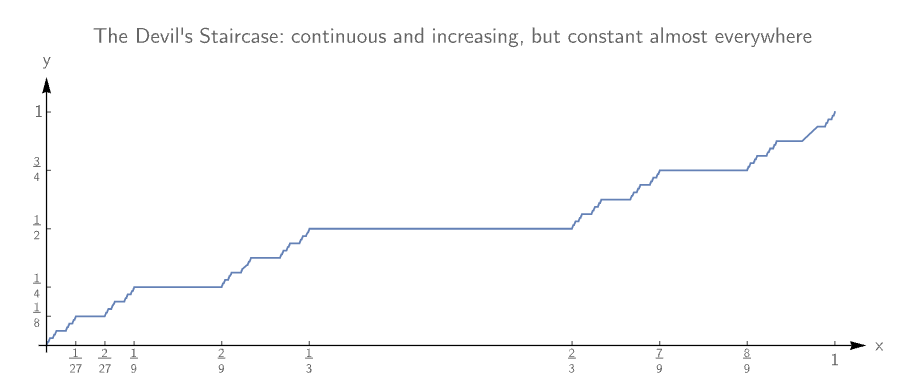
\includegraphics[width=0.5\textwidth]{dev.png}}
        \subfigure[The Riemann Function]{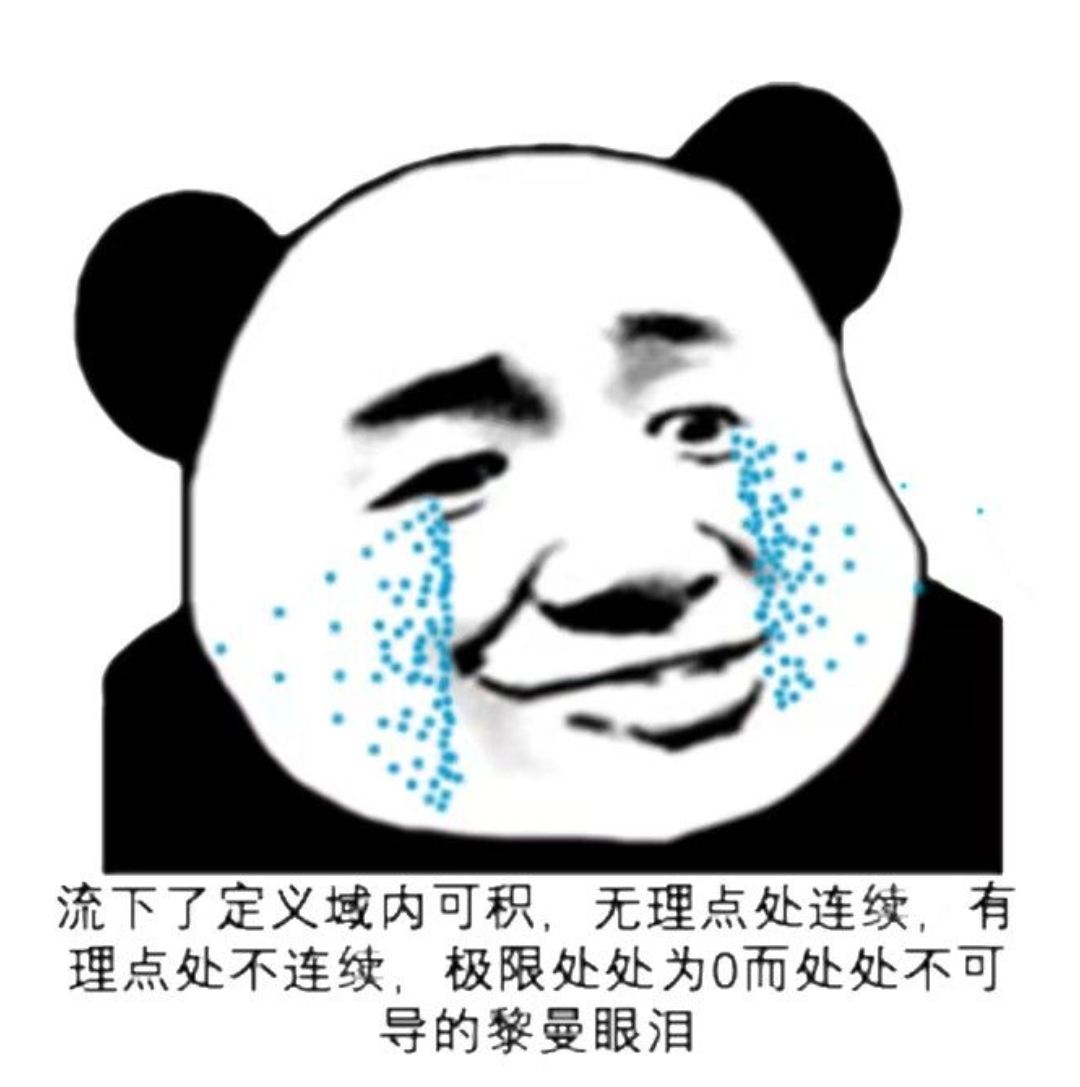
\includegraphics[width=0.4\textwidth]{Re.jpg}}
    \end{figure}
    

\end{frame}
\begin{frame}
    \frametitle{Results/Theorems for Continuous Real Functions}
    \begin{itemize}
        \item[(1)] Let $\Omega\subset\mathbb{R}$ be some set and $f:\Omega\to \mathbb{R}$ be a function
         that is continuous at some point $x_0 \in \Omega$  and assume that $f(x_0)>0$. 
         Then there exists a $\delta>0$ such that $f(x)>0$ for all $x \in (x_0-\delta,x_0+\delta)\cap \Omega$. (Slide 227)
        \item[(2)] Let $a<b$ and $f:[a,b]→\mathbb{R}$ be a continuous function with $f(a)<0<f(b)$. 
        Then there exists some $x \in [a,b]$ such that $f(x)=0$. (Slide 228)
        \item[(3)] Let $a<b$ and $f:[a,b]→\mathbb{R}$ be a continuous function. 
        Then for $y \in [\min\{f(a),f(b)\},\max \{f(a),f(b)\}]$ there exists some $x \in [a,b]$ such that $y=f(x)$. (Slide 230)
    \end{itemize}
\end{frame}
\begin{frame}
    \frametitle{Results/Theorems for Continuous Real Functions}
    \begin{itemize}
        \item[(4)] Let $f:[a,b]\to \mathbb{R}$ be a continuous function with $ran~f\subset[a,b]$. 
        Then $f$ has a fixed point, i.e., there exists some $x \in [a,b]$ such that $f(x)=x$. (Slide 231) 
        \item[(5)] Let $\Omega \subset \mathbb{R}$ be some set and $𝑓:\Omega\to \mathbb{R}$ be a function 
        that is continuous at some point $x_0 \in \Omega$. Then there exists a $\delta > 0$ such that 
        $f$ is bounded above on $(x_0-\delta,x_0+\delta)\cup\Omega$. (Slide 233) 
        \itshape Comment: This Lemma mainly deals with the behavior of $f$ locally (on some neighborhood) 
        \myfont
        \item[(6)] Let $a < b$ and $f:[a,b]\to \mathbb{R}$ be a continuous function. 
        Then $f$ is bounded above. (Slide 234) 
    \end{itemize}
\end{frame}
\begin{frame}
    \frametitle{Results/Theorems for Continuous Real Functions}\
    \begin{itemize}
        \item[(7)] Let $a < b$ and $f:[a,b]\to \infty$ be a continuous function. 
        Then there exists a $y \in [a,b]$ such that $f(x)\leq f(y)$ for all $x \in [a,b]$. (Slide 236) 
        \itshape Comment. This theorem ensures that $f$ takes its maximum and minimum on $[a,b]$. \myfont
        \item[(8)] Let $f:I \to \mathbb{R}$ be a continuous function, where $I$ is an interval. 
        Then $f$ is strictly monotonic if and only if $f$ is bijective. (Slide 240 \& 244) 
        \item[(9)] Let $f:I\to \mathbb{R}$ be a continuous function. Suppose $[a,b]\subset I$, then $f([a,b])$ is an interval. (Slide 251)
    \end{itemize}
    \vspace{1em}
    \textcolor{red}{They are important! Make sure you have time to digest these!}
\end{frame}
\begin{frame}
    \frametitle{Uniform continuity}
    Interpretation: \textcolor{brown}{not driving to fast!}\\ 
    Example: $f(x)=\sin \frac{1}{x}$ on the interval (0,1) is not uniformly continuous
    \vspace{2em}\\
    Uniform Continuty Theorem:\\
    Let $f:I\to\mathbb{R}$ be a continuous function. 
    Suppose $[a,b]\subset I$, then $f$ is uniformly continuous on $[a,b]$.  (Slides 249)

\end{frame}
\section{Exercises}
\begin{frame}
    \frametitle{Exercises}
    1. Discuss where is the following function continuous, where is it not continuous. 
    No proof needed.  \\
    \begin{itemize}
        \item[(i)]$f(x)=\frac{\sqrt{3}{(1+4x)}-1}{2\sin x}$ 
        \item[(ii)]$f(x)= \lceil x\rceil, x>0$ 
    \end{itemize}
      (Adapted from SJTU Math textbook, P69)
    
    \vspace{8em}
    \tiny{(It’s necessary to being able to investigate concrete functions)}
\end{frame}
\begin{frame}
    \frametitle{Exercises}
    2. Please prove, or disprove by giving counterexamples of the following statements: 
    \begin{itemize}
        \item [(i)]  $(1+O(x))^2=1+O(x^2)$ as $x\to 0$ 
        \item [(ii)]  $o(x)^n=o(x^n), n \in \mathbb{N}^*$, as $x \to0$
    \end{itemize}

    \vspace{3em}
    What about $x \to \infty$ ? Would the result change?
\end{frame}
\begin{frame}
    \frametitle{Exercises}
    3. Let $f:[0,+\infty)\to \mathbb{R}$ be a continuous function such that 
    $\underset{x\to \infty}{\lim}⁡ f(x)$ exists and is finite. 
    Show that $f$ is uniformly continuous on $[0, +\infty)$.


\end{frame}
\begin{frame}
    \frametitle{Exercises}
    4. Let $f:[a,b]\to \mathbb{R}$ be a continuous function with $b>a$. 
    Given $\varepsilon>0$, show that there is a polygonal function $g$ such that 
    $|f(x)-g(x)|<\varepsilon$ for all $x \in [a,b]$.\\
    \vspace{3em}
    Note: A polygonal function is a function formed by a finite number of line segments.
     Of course, a polygonal function is continuous. 
    
    \vspace{2em}
    \begin{itemize}
        \item \textcolor{red}{Try to write a complete proof!}
    \end{itemize}
\end{frame}
\begin{frame}
    \frametitle{Exercises}
    5$^*$. The function $f(x)$ is defined on interval $I$. Proof that $f(x)$ is uniformly continuous
    if and only if: for any sequence ${x_n'},{x_n''}\subset I$, if $\underset{n \to \infty}{\lim}(x_n'-x_n'')=0$,
    then $\underset{n \to \infty}{\lim}(f(x_n')-f(x_n''))=0$.
\end{frame}
\begin{frame}
    \frametitle{Exercises}
    6$^*$.Let $f:(0,+\infty)\to\mathbb{R}$ be a continuous function such that 
    $f(x^2)=f(x)$. Please show that $f$ is a constant function on $(0,+\infty)$
    , i.e., $$\exists M \in \mathbb{R},  \forall x \in dom f, f(x)=M$$
    (SJTU Math textbook, P70)

\end{frame}
\begin{frame}
    \frametitle{Exercises}
    7$^*$. Suppose the right endpoint for an interval $I_1$ is $c\in I_1$, the left endpoint
    for an interval $I_2$ is also $c\in I_2$($I_1, I_2$ can be infinite interval or just finite). Prove that
    if $f$ is uniformly continuous on $I_1$ and $I_2$, then f is uniformly continuous on $I=I_1\cup I_2$.

\end{frame}
\begin{frame}
    \frametitle{Exercises}
    8. Let $f:\Omega \to \mathbb{R}$ be a real function that satisfies \textcolor{blue}{Lipschitz condition}, that is, 
    there is a constant $M>0$ such that for all $x$ and $y$ in the domain of $f$, $|f(x)-f(y)|\leq M∙|x-y|$.\\
    \vspace{1em}
    \begin{itemize}
        \item [(i)]Show that $f$ is uniformly continuous
        \item [(ii)] Now Let $\Omega=:[a, +\infty)$, where $a>0$. Show that $f(x)/x$ is uniformly continuous
    \end{itemize} 

\end{frame}
\section{Appendix}
\begin{frame}
    \frametitle{Intergration Bee!}
    Horst and My TAs plan to hold 2-nd \textcolor{blue}{JI Intergration Bee} this semester, probably in early November. 
    The problems would include:
    \begin{itemize}
        \item single variable intergration(you'll learn this in vv186).
        \item multi variable intergration(e.g. surface intergal, learn in vv285)
        \item ordinary differential equations(learn in vv286).
    \end{itemize}
    \vspace{2em}
    If you're interested, feel free to contact us!
\end{frame}
\begin{frame}
    \frametitle{Midterm Reminder}
    \begin{itemize}
        \item The first midterm exam is scheduled onto next Tuesday, lecture time.
        \item Big RC and OH will be held on Sunday (time will be announced
        later).
        \item Tips for reviewing:
        \begin{itemize}
            \item[1.] Go through the lecture slides. Recite the definitions and theorem
            statements. If time permits, review the proofs of theorems and
            lemmas.
            \item[2.] Go through the assignments. Pay attention to the definitions in
            them ($\varlimsup$, $\varliminf$, etc.)
            \item[3.] Do the sample exams and check the answers.
            \item[4.] Attend the big RC unless you are very confident.        
        \end{itemize}
        \item \textcolor{red}{Remember to sleep well the night before the exam!}
        \item Good luck!
    \end{itemize}
    

\end{frame}
\begin{frame}
    \frametitle{Reference}
    \begin{itemize}
        \item Exercises from 2019–Vv186 TA-Zhang Leyang.
        \item Exercises from 2020-Vv186 TA-Hu Pingbang.
        \item SJTU Math Textbook.
        \item Mathmatical Analysis I. \itshape Department of Mathematics, ECNU,\myfont
        ,4-th version. Beijing: Higher Education Press. 2016.3 print.
    \end{itemize}

\end{frame}
\end{document}